\subsection{Uncontrolled dynamics}

The uncontrolled dynamics of the satellite is simulated for one orbital period (equal to $\approx 1.54$ hours). The starting time is set to $t_0 = 0 \,s$. The initial conditions are the following:
\begin{equation*}
    \bm{\omega}_0 = \begin{bmatrix}
    20 & 14 & 3
    \end{bmatrix}^T \;
    ^{\circ}/s, \qquad
    q_0 = \begin{bmatrix}
    0 & 0 & 0 & 1
    \end{bmatrix}^T, \qquad
    \theta_0 = 0^{\circ}, \qquad
    \Bar{\mathbf{M}}_{d,0} = \begin{bmatrix}
    0 & 0 & 0
    \end{bmatrix}^T \; N \cdot m
\end{equation*}

The evolution in time of the disturbing torques, of the angular velocity and of the attitude quaternion are reported in \cref{fig:uncontrolled-disturbances,fig:uncontrolled-wq}.

\begin{figure}[h!]
    \centering
    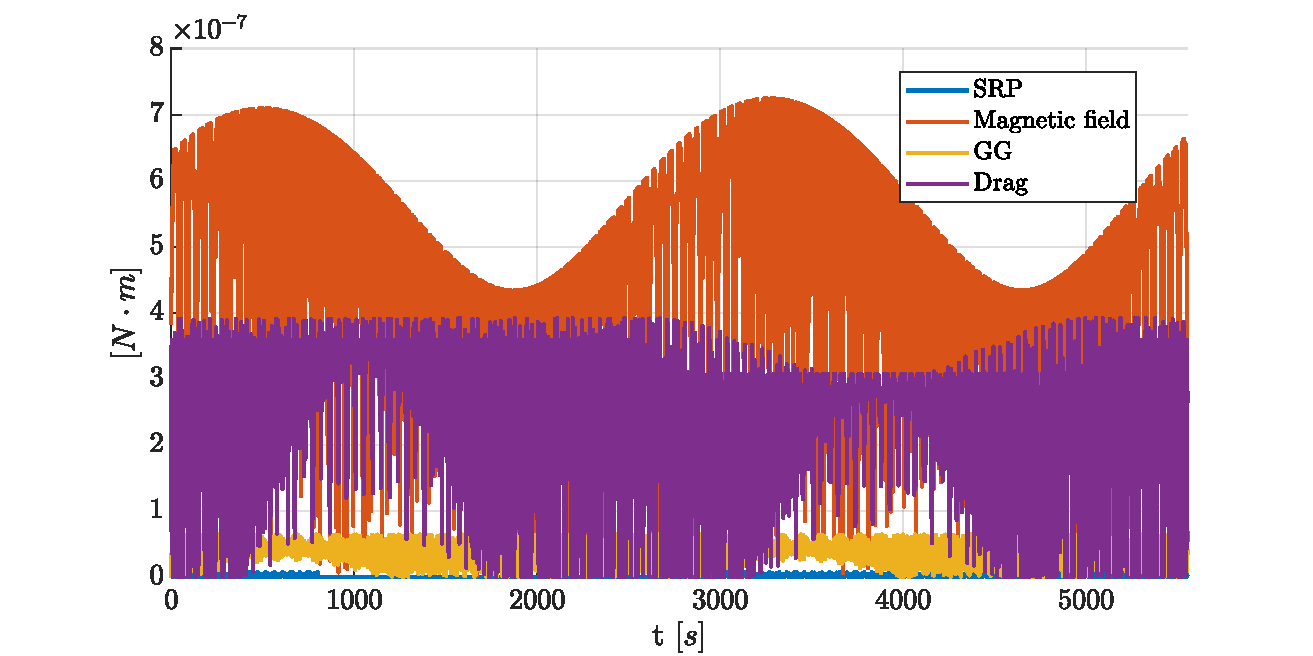
\includegraphics[width=0.8\textwidth]{graphics/uncontrolled/uncontrolled-disturbances.pdf}
    \caption{Evolution of the disturbances acting on the spacecraft}
    \label{fig:uncontrolled-disturbances}
\end{figure}

\begin{figure}[h!]
    \centering
    \subfloat[Angular velocity]{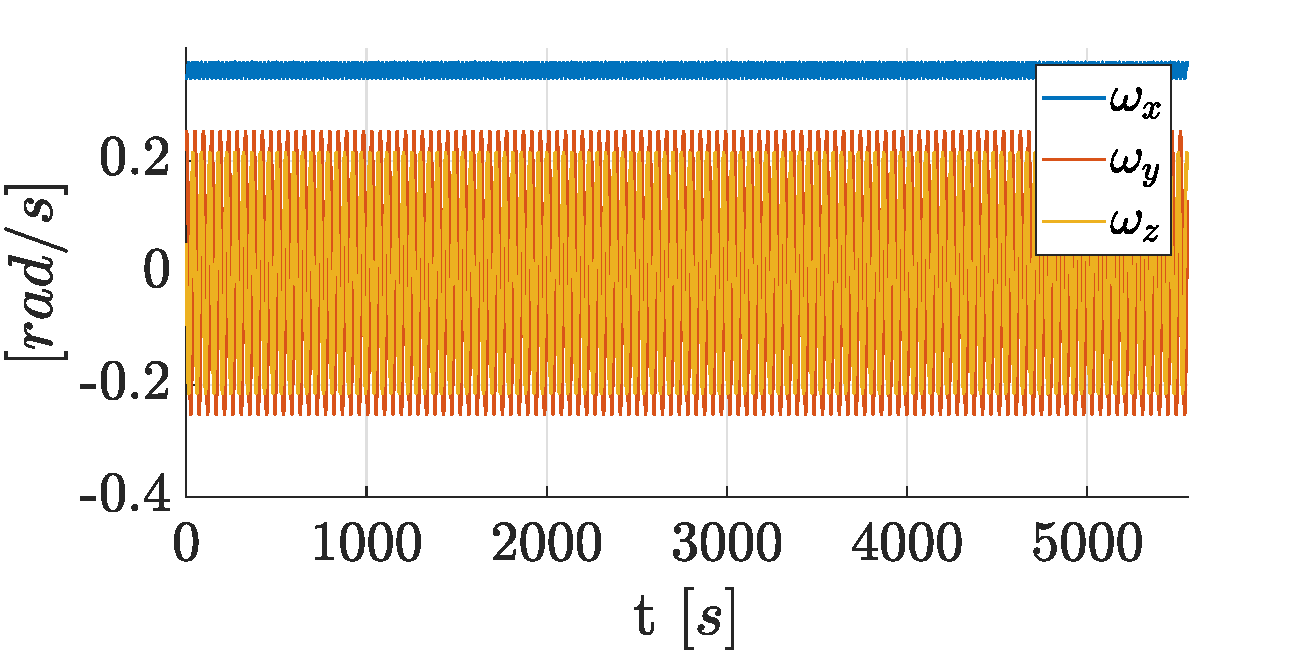
\includegraphics[width=0.49\textwidth]{graphics/uncontrolled/uncontrolled-w.pdf}}
    \subfloat[Quaternion]{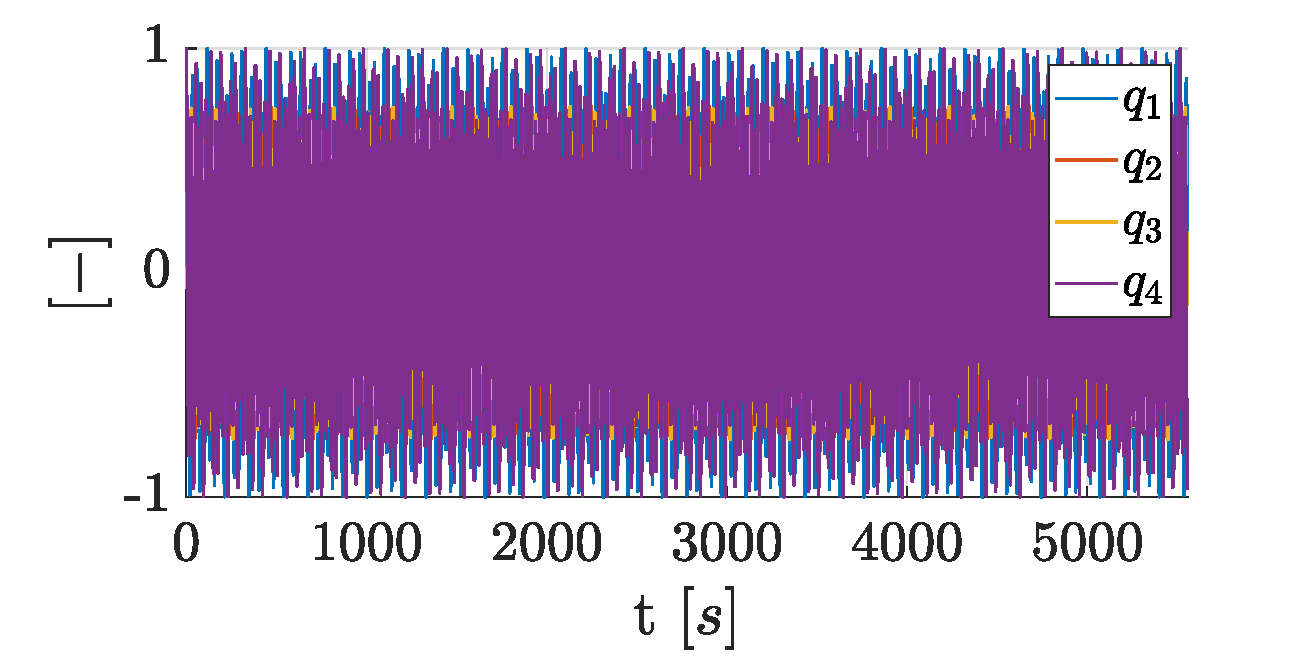
\includegraphics[width=0.49\textwidth]{graphics/uncontrolled/uncontrolled-q.pdf}}
    \caption{Evolution of $\bm{\omega}$ and $q$ in uncontrolled dynamics}
    \label{fig:uncontrolled-wq}
\end{figure}

\cref{tab:magnitude_torques} reports the maximum magnitude of the four disturbing torques. It is clear from the latter (as it also was from \cref{fig:uncontrolled-disturbances}) that the main disturbances are due to the magnetic field and the atmosphere, as the altitude of the orbit is relatively low. The impact that the gravity gradient and SRP have on the rotational dynamics is smaller.


\begin{table}[h!]
    \centering
    \caption{Maximum magnitude of the disturbing torques}
    \begin{tabular}{ccccc}
    \toprule
    \toprule
    & $\mathbf{M}_{\mathbf{b}}$ & $\mathbf{M}_{GG}$ & $\mathbf{M}_{drag}$ & $\mathbf{M}_{SRP}$\\
    \midrule
    Max. magnitude [$N\cdot m$] & 7.24 $\cdot 10^{-7}$ & 6.47 $\cdot 10^{-8}$ & 3.92 $\cdot 10^{-7}$ & 7.55 $\cdot 10^{-9}$ \\
    \bottomrule
    \bottomrule
    \end{tabular}
    \label{tab:magnitude_torques}
\end{table}

\subsection{Detumbling} \label{sec:control-tracking}

The detumbling phase is simulated from $t_0 = T = 5555.32 \, s$ to $t_{end} = 22220.93 \, s$. The initial conditions for both control strategies are set equal to:

\begin{equation*}
    \bm{\omega}_0 = \begin{bmatrix}
    21.10 & 7.38 & 10.55
    \end{bmatrix}^T \;
    ^{\circ}/s, \qquad
    q_0 = \begin{bmatrix}
    -0.17 & -0.15 & -0.14 & -0.96
    \end{bmatrix}^T, \qquad
    \theta_0 = 0^{\circ}
\end{equation*}
\begin{equation*}
    \Bar{\mathbf{M}}_{d,0} = \begin{bmatrix}
    0.03 & 0.12 & 0.49
    \end{bmatrix}^T \cdot 10^{-4} \, N \cdot m, \qquad
    \mathbf{h}_{r,0} = \begin{bmatrix}
    0 & 0 & 0 & 0
    \end{bmatrix}^T \; kg \, m^2/s
\end{equation*}

The results of the evolution of the angular velocity and of the attitude quaternions for both controls are presented in \cref{fig:detumbling-w,fig:detumbling-q}.

\begin{figure}[h!]
    \centering
    \subfloat[Spin rate damping]{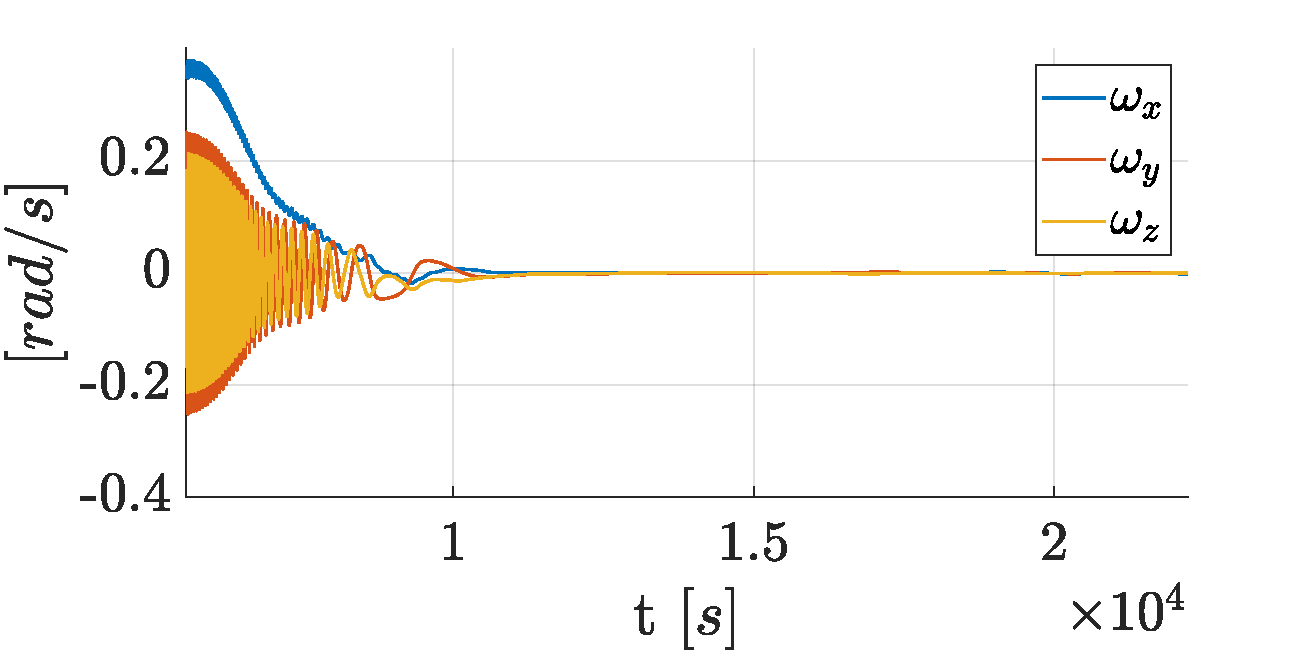
\includegraphics[width=0.49\textwidth]{graphics/detumbling-SRD/detumblingSRD-w.pdf}}
    \subfloat[Proportional control]{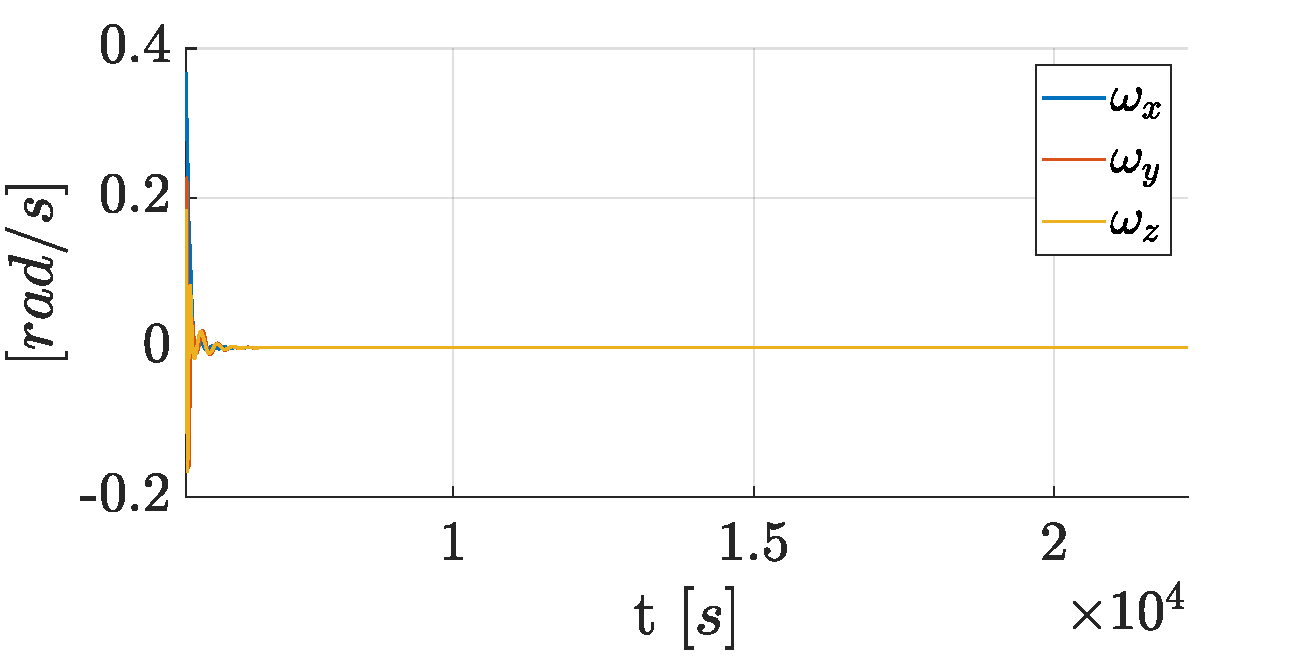
\includegraphics[width=0.49\textwidth]{graphics/detumbling-P/detumblingP-w.pdf}}
    \caption{Evolution of $\bm{\omega}$ in the detumbling phase}
    \label{fig:detumbling-w}
\end{figure}

\begin{figure}[h!]
    \centering
    \subfloat[Spin rate damping]{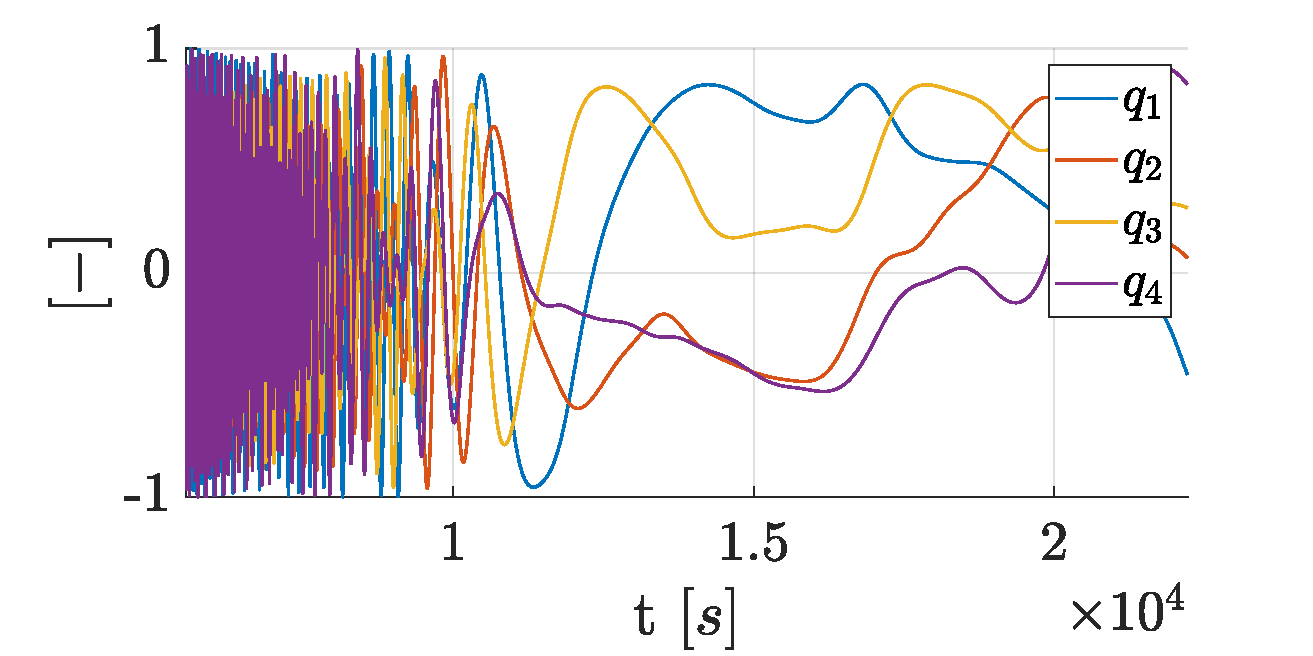
\includegraphics[width=0.49\textwidth]{graphics/detumbling-SRD/detumblingSRD-q.pdf}}
    \subfloat[Proportional control]{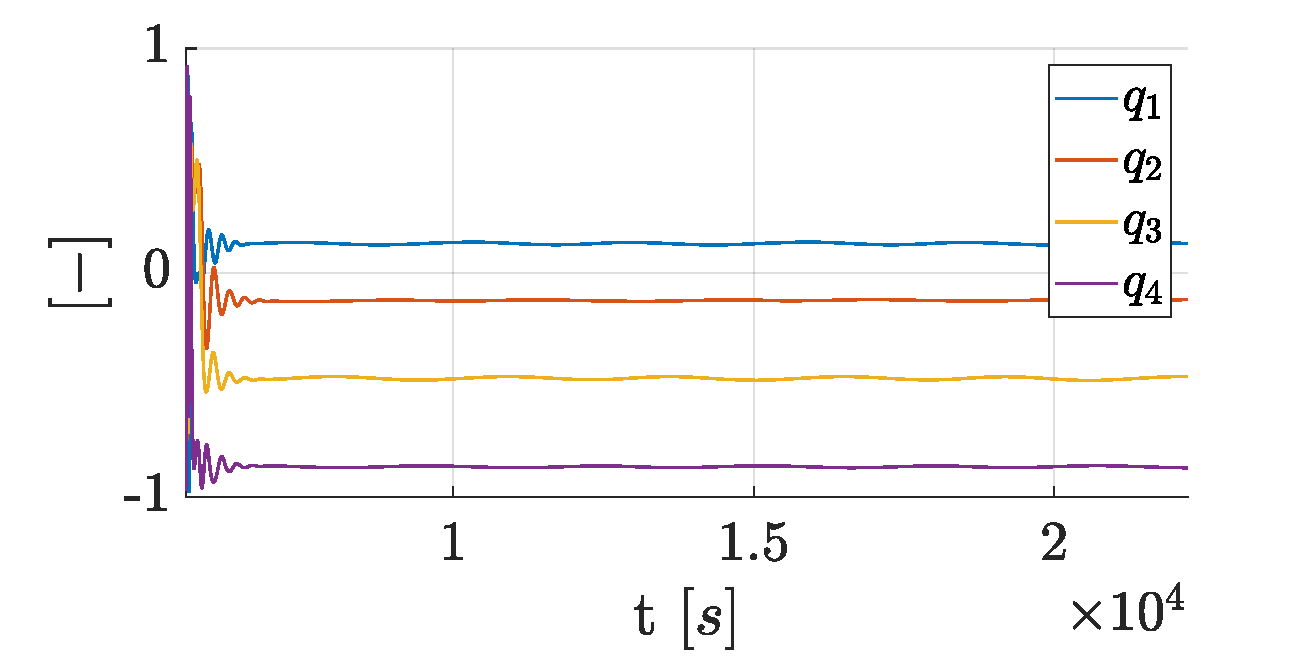
\includegraphics[width=0.49\textwidth]{graphics/detumbling-P/detumblingP-q.pdf}}
    \caption{Evolution of $q$ in the detumbling phase}
    \label{fig:detumbling-q}
\end{figure}

The proportional control proves to be more efficient: $\bm{\omega}$ quickly drops close to zero and the attitude quaternion stabilizes itself after $\approx 1000 \, s$. In the spin rate damping, the detumbling can be considered to be completed in $\approx 5500 \, s \approx 1\, T$. All the components of the angular velocity face a slower decay compared to the other strategy: this is due to the inherent nature of the magnetorquer, which is less powerful than the RWs and can rarely generate the required control torque, as explained in \cref{sec:control}. The values of the angular velocity at the end of the control phase are reported in \cref{tab:detumbling_finalW}. It is clear again that the proportional control guarantees better performances.

\begin{table}[h!]
    \centering
    \caption{Values of the angular velocity after the detumbling phase}
    \begin{tabular}{cc}
    \toprule
    \toprule
    \multicolumn{2}{c}{\textbf{$\bm{\omega}$ after the detumbling control} $[rad/s]$} \\
    \midrule
    Spin rate damping & Proportional control \\
    \midrule
    $\begin{bmatrix} -16.21 & 0.01 & -0.03 \end{bmatrix}^T \cdot 10^{-2}$  &  $\begin{bmatrix} 0.15 & -0.21 & 0.09 \end{bmatrix}^T \cdot 10^{-4}$ \\
    \bottomrule
    \bottomrule
    \end{tabular}
    \label{tab:detumbling_finalW}
\end{table}

The performances of the QUEST estimator and of the ESO are presented through the plots in \cref{fig:detumbling-estQ,fig:detumbling-estW}. In both strategies, the estimation of both $q$ and $\bm{\omega}$ is not satisfactory in the first time instants. The error on the attitude quaternion goes below $10^{-4}$ in $\approx 200 \,s$ for the proportional control, while for the SRD the same value is reached only after $\approx 2700 \,s$. The fact that the decay rate of the error is different for the two strategies could be attributed to the higher frequency of oscillation of $\bm{\omega}$ in the first part of the SRD compared the proportional control. The time variations of the quaternion are very fast, so the sensors for the attitude determination (especially the star tracker, whose update rate is slow) might not keep up at generating updated measurements, degrading the performances of the QUEST algorithm. The same phenomenon can be noticed in the estimation of the angular velocity: for the proportional control, the error drops close to $10^{-3}\, rad/s$ after $1000\, s$, while in the SRD it takes $\approx 2700 \,s$. The decay of the error on the angular velocity is slower with respect to the estimation of $q$ as $\bm{\omega}$ goes through multiple steps in its determination (low-pass filtering of $\Bar{q}$ $\rightarrow$ numerical derivation of $\Bar{q}$ $\rightarrow$ ESO), while the quaternion is a direct product of the QUEST algorithm.

\begin{figure}[h!]
    \centering
    \subfloat[Spin rate damping]{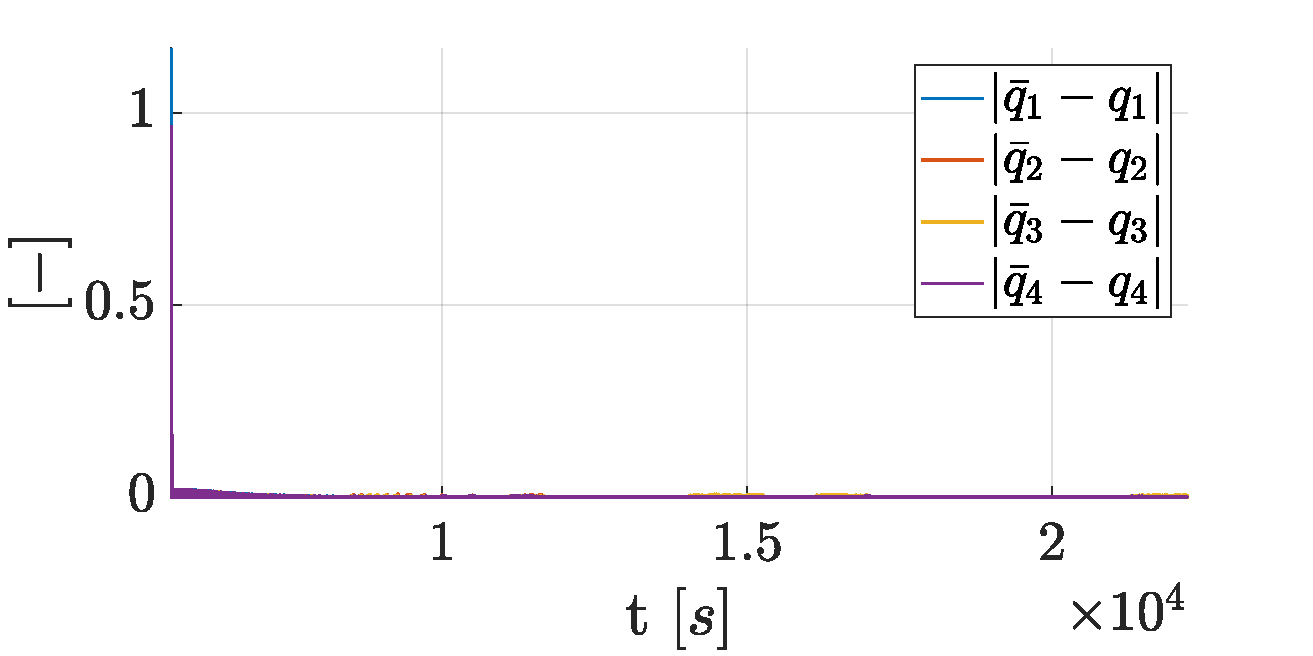
\includegraphics[width=0.49\textwidth]{graphics/detumbling-SRD/detumblingSRD-estQ.pdf}}
    \subfloat[Proportional control]{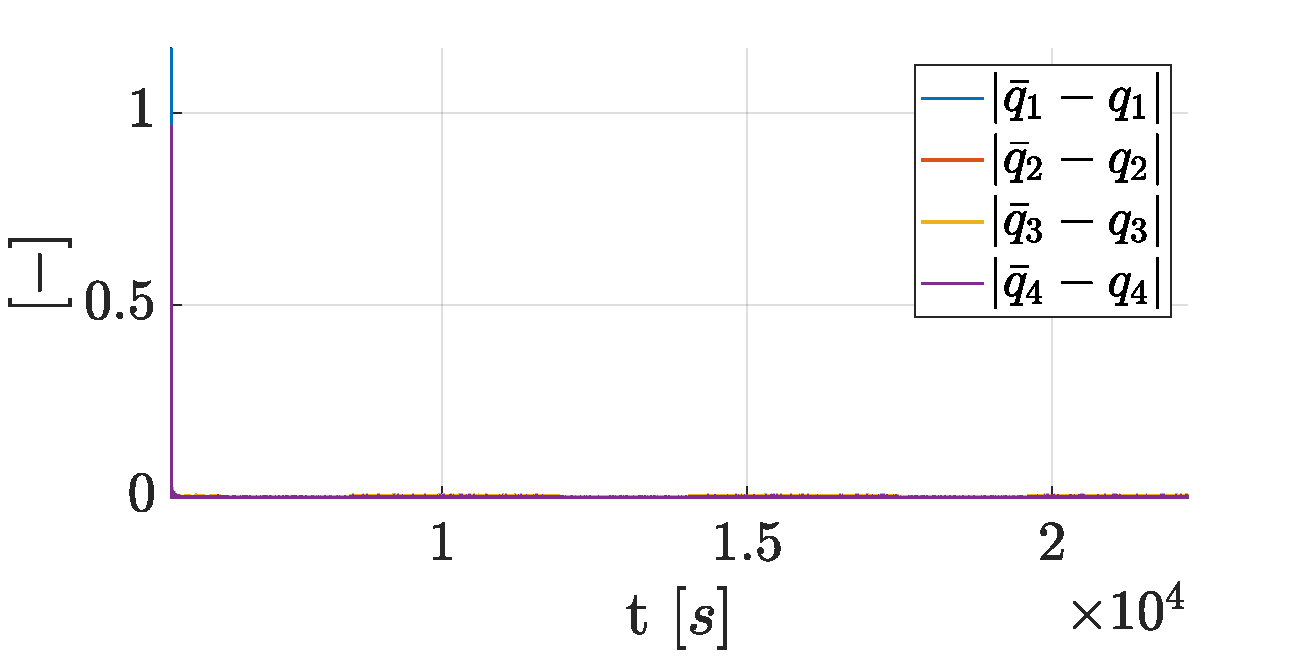
\includegraphics[width=0.49\textwidth]{graphics/detumbling-P/detumblingP-estQ.pdf}}
    \caption{Evolution of the estimation error on $q$ in the detumbling phase}
    \label{fig:detumbling-estQ}
\end{figure}

\begin{figure}[h!]
    \centering
    \subfloat[Spin rate damping]{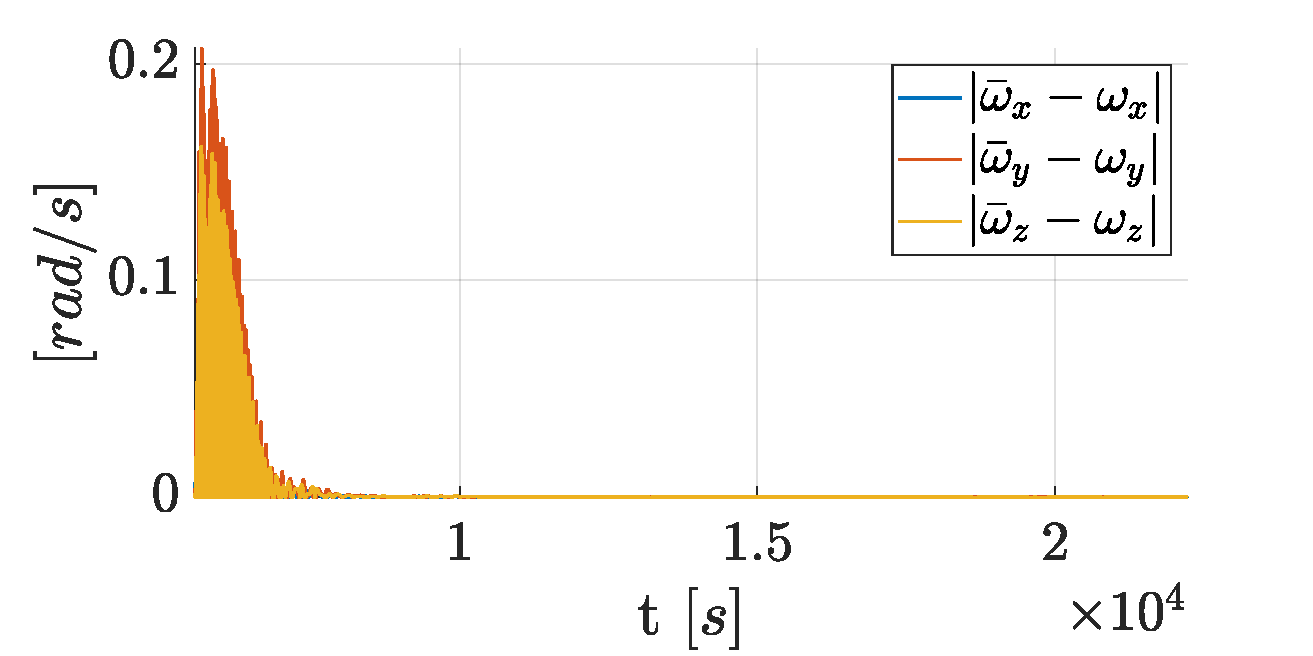
\includegraphics[width=0.49\textwidth]{graphics/detumbling-SRD/detumblingSRD-estW.pdf}}
    \subfloat[Proportional control]{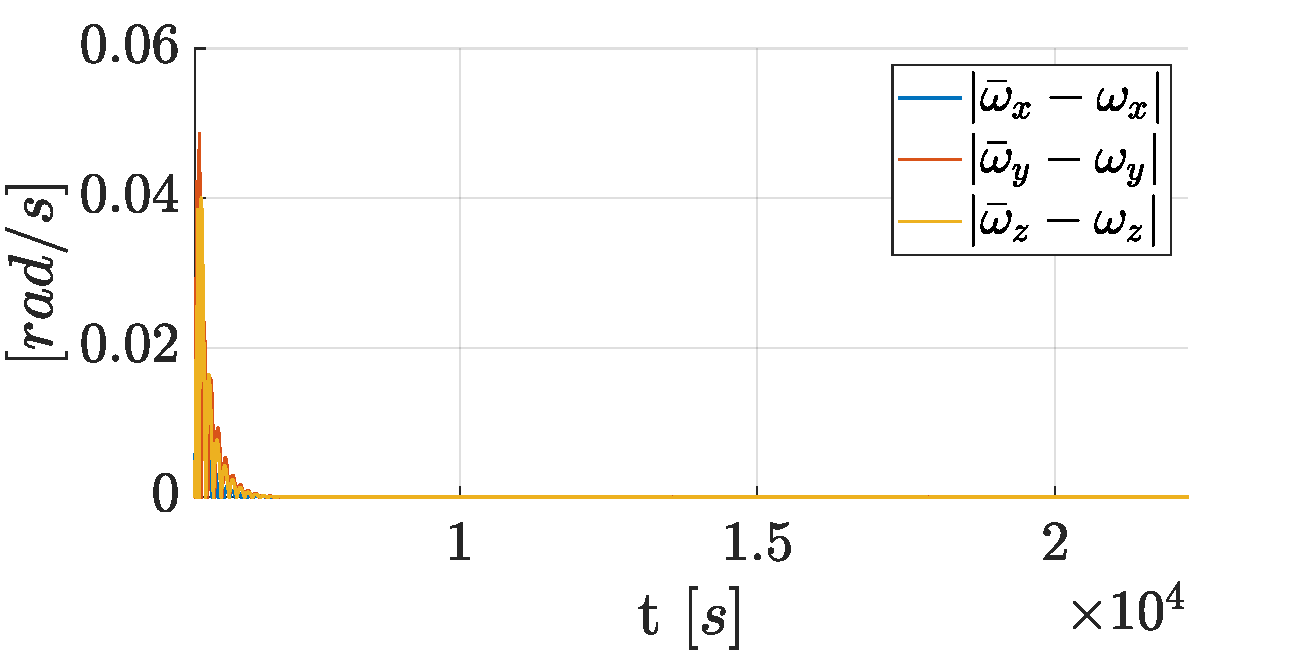
\includegraphics[width=0.49\textwidth]{graphics/detumbling-P/detumblingP-estW.pdf}}
    \caption{Evolution of the estimation error on $\bm{\omega}$ in the detumbling phase}
    \label{fig:detumbling-estW}
\end{figure}

\cref{fig:detumblingSRD-D} reports the values of the components of the magnetic dipole which the magnetorquer must generate in the spin rate damping. The actuator gets saturated in all the three directions in the first part of the control.

\begin{figure}[h!]
    \centering
    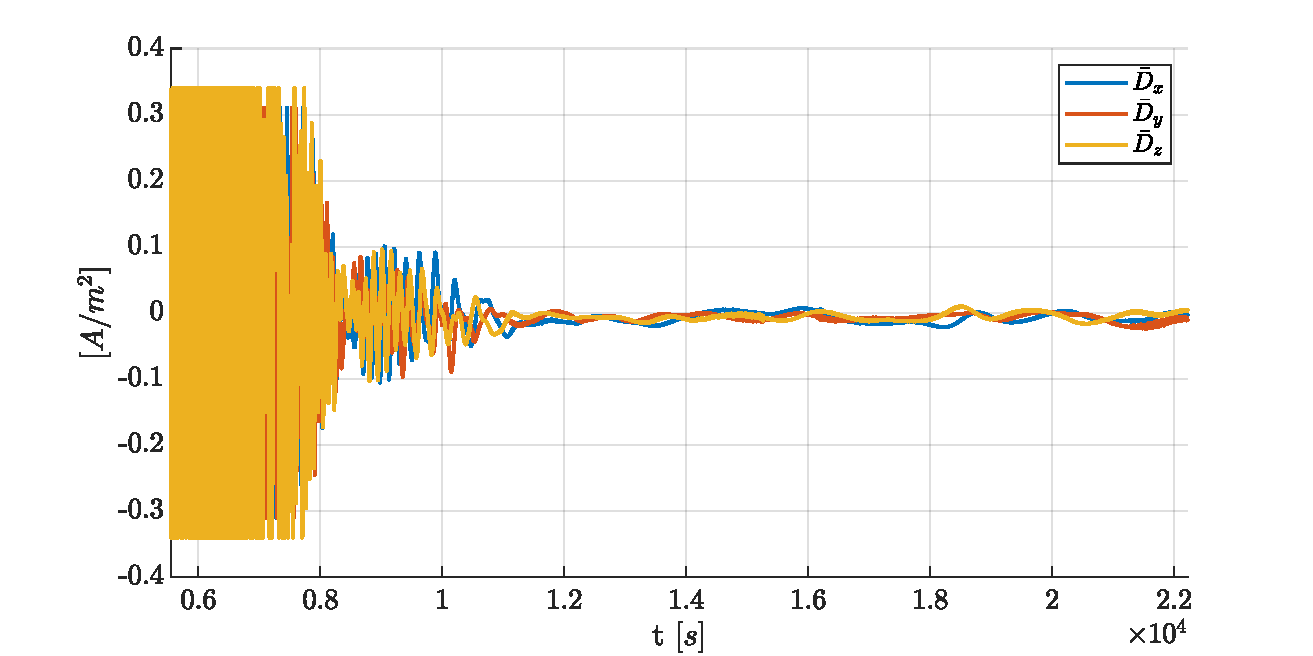
\includegraphics[width=0.8\textwidth]{graphics/detumbling-SRD/detumblingSRD-D.pdf}
    \caption{Evolution of the magnetic dipole of the magnetorquer}
    \label{fig:detumblingSRD-D}
\end{figure}

\subsection{Tracking}

The tracking phase is simulated from $t_0 = 22220.93 \, s$ to $t_{end} = 38886.63 \, s$. The initial conditions for this simulation are retrieved from the final conditions of the detumbling phase with the proportional control.

\begin{equation*}
    \bm{\omega}_0 = \begin{bmatrix}
    0.15 & -0.21 & 0.09
    \end{bmatrix}^T \cdot 10^{-4} \;
    rad/s, \qquad
    q_0 = \begin{bmatrix}
    0.13 & -0.11 & -0.46 & -0.86
    \end{bmatrix}^T, \qquad
    \theta_0 = 0^{\circ}
\end{equation*}
\begin{equation*}
    \Bar{\mathbf{M}}_{d,0} = \begin{bmatrix}
    -0.08 & -0.05 & -0.46
    \end{bmatrix}^T \cdot 10^{-6} \, N \cdot m, \qquad
    \mathbf{h}_{r,0} = \begin{bmatrix}
    -1.14 & 16.52 & 13.6 & -4.06
    \end{bmatrix}^T \; mN \cdot ms
\end{equation*}

The results of the simulations are presented in the plots below. It is clear from \cref{fig:tracking-w} and \cref{fig:tracking-Abn_pe} that the control logic fulfils the requirements. The first two components of the angular velocity quickly drop to zero, while the third one tracks the angular speed of the LVLH frame $\Dot{\theta}$: as it is possible to see in \cref{fig:tracking-w_zoom}, $\omega_z$ oscillates around the orbital mean motion $n = 1/T$. The evolution of direction cosines becomes periodic. The pointing error decays rapidly, reaching values close to $10^{-3}\,{}^{\circ}$ in approximately $1300 \, s$, thus satisfying the mission requirements.

\begin{figure}[h!]
    \centering
    \subfloat[Angular velocity]{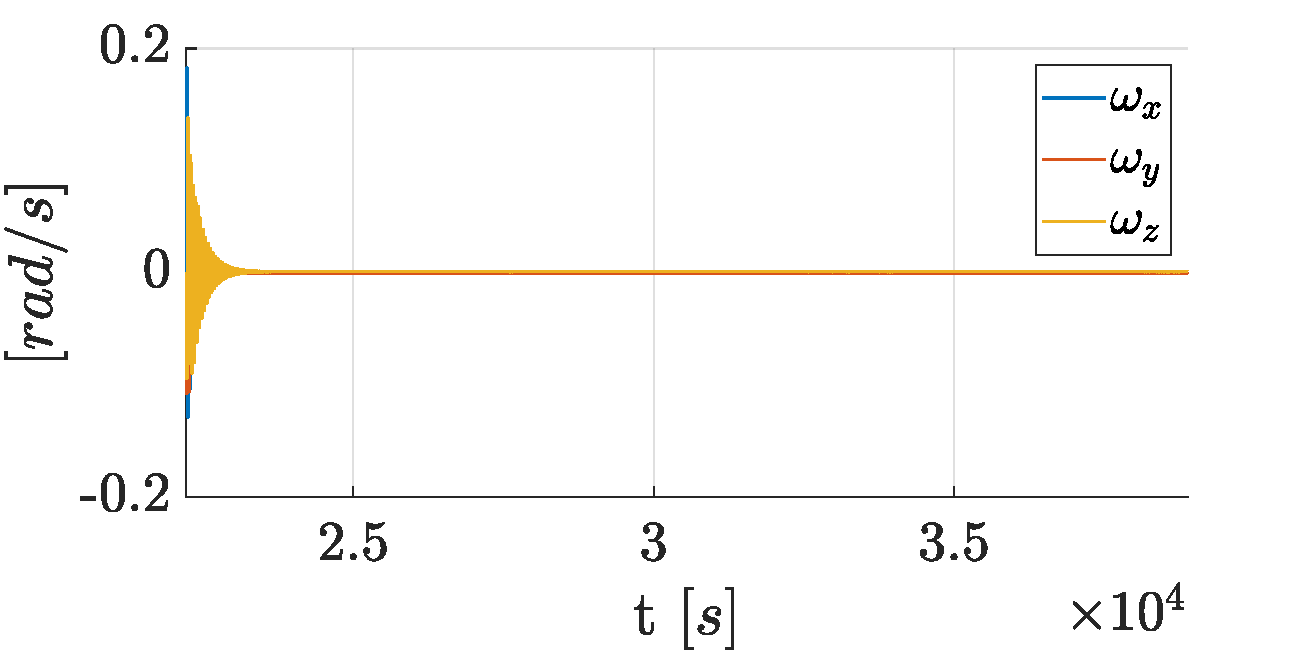
\includegraphics[width=0.49\textwidth]{graphics/tracking/tracking-w.pdf}}
    \subfloat[Angular velocity (detail) \label{fig:tracking-w_zoom}]{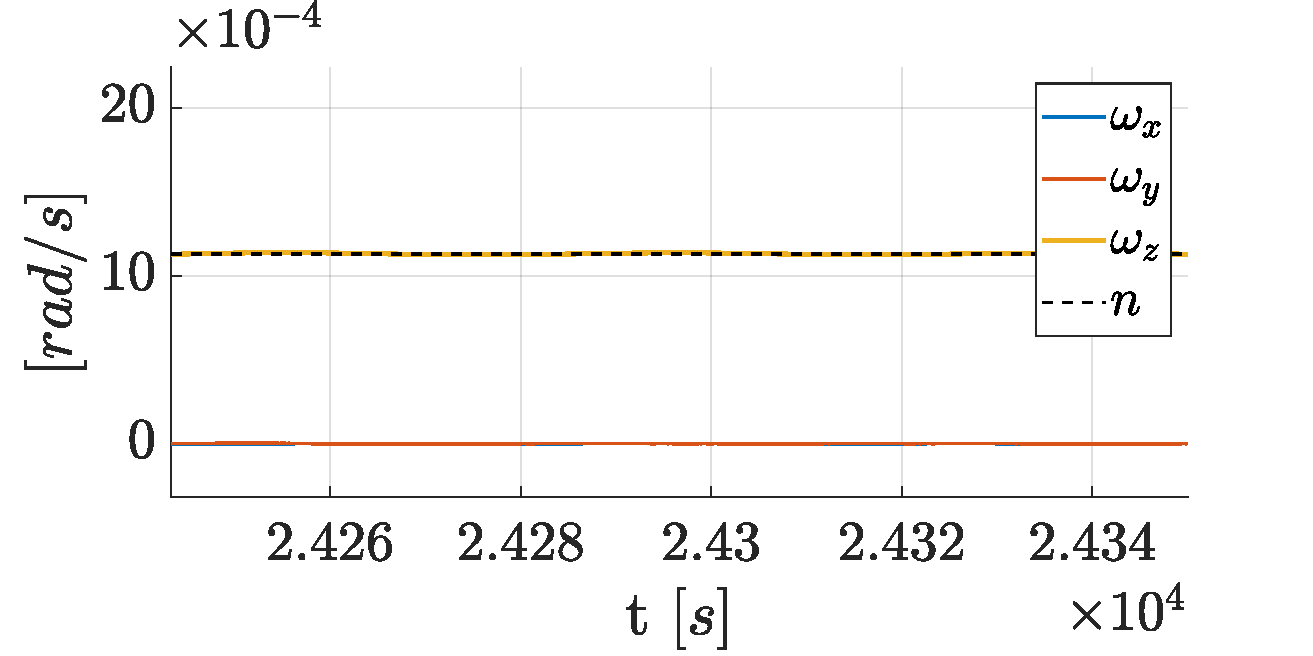
\includegraphics[width=0.49\textwidth]{graphics/tracking/tracking-w_zoom.pdf}}
    \caption{Evolution of $\bm{\omega}$ in the tracking phase}
    \label{fig:tracking-w}
\end{figure}

\begin{figure}[h!]
    \centering
    \subfloat[Direction cosines matrix]{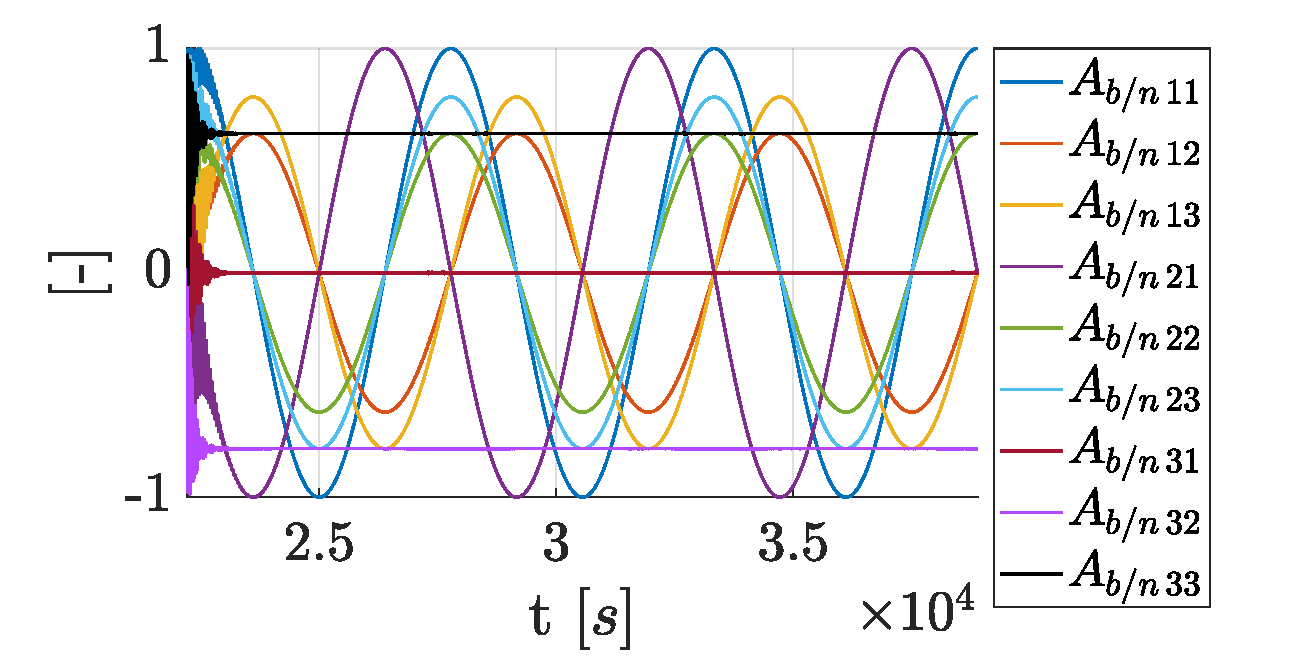
\includegraphics[width=0.49\textwidth]{graphics/tracking/tracking-Abn.pdf}}
    \subfloat[Pointing error]{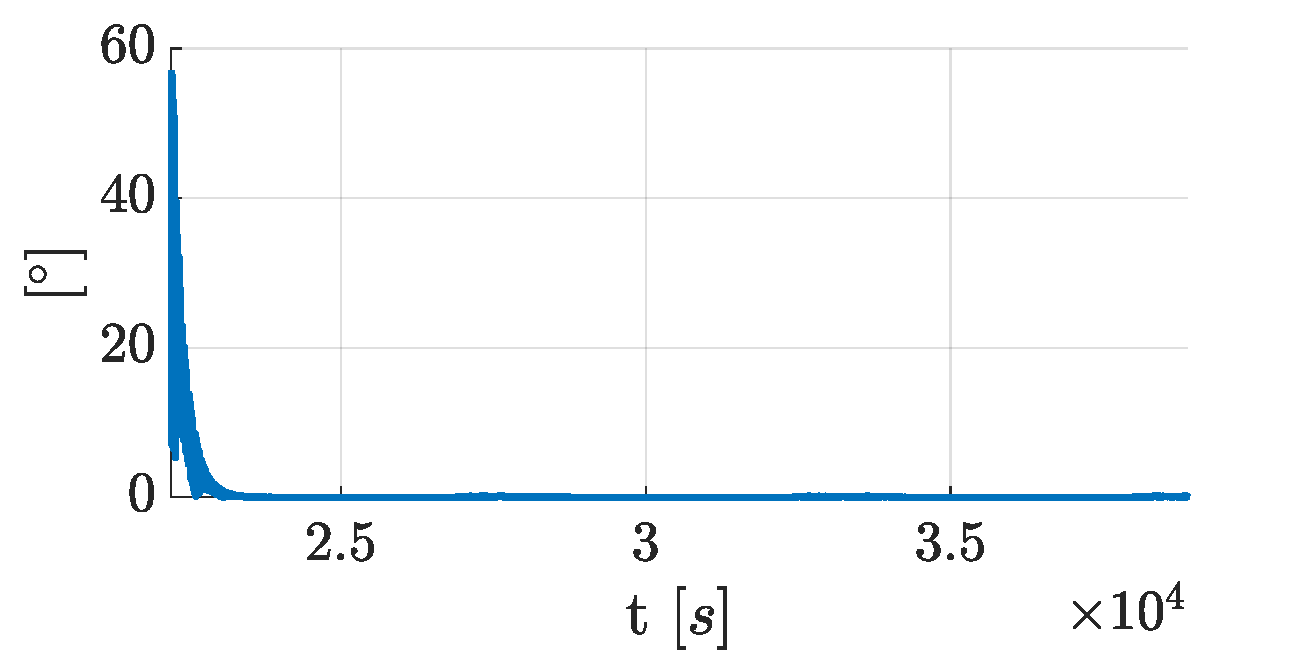
\includegraphics[width=0.49\textwidth]{graphics/tracking/tracking-pe.pdf}}
    \caption{Evolution of $A_{b/n}$ and of the pointing error in the tracking phase}
    \label{fig:tracking-Abn_pe}
\end{figure}

For this phase, the performance of the estimators (QUEST + ESO) are presented through the plots in \cref{fig:tracking-estWabn}. The errors associated to the direction cosines matrix (\cref{fig:tracking-estAbn}), which is derived directly from the QUEST method via \cref{eq:dcm}, rapidly drop to zero. The estimation of the angular velocity becomes satisfactory only after $\approx 1200 \, s$ (with $\| \bar{\bm{\omega}} - \bm{\omega} \|$ in the order of $10^{-5} \, rad/s$). The reasons of this behaviour are the same as the ones explained in \cref{sec:control-tracking}. The same trend can be observed also in the estimations of the disturbing and control torques (\cref{fig:tracking-estMd,fig:tracking-estMc}), as they come from the dynamics of the ESO which involves $\bar{\bm{\omega}}$. 

\begin{figure}[h!]
    \centering
    \subfloat[Direction cosine matrix \label{fig:tracking-estAbn}]{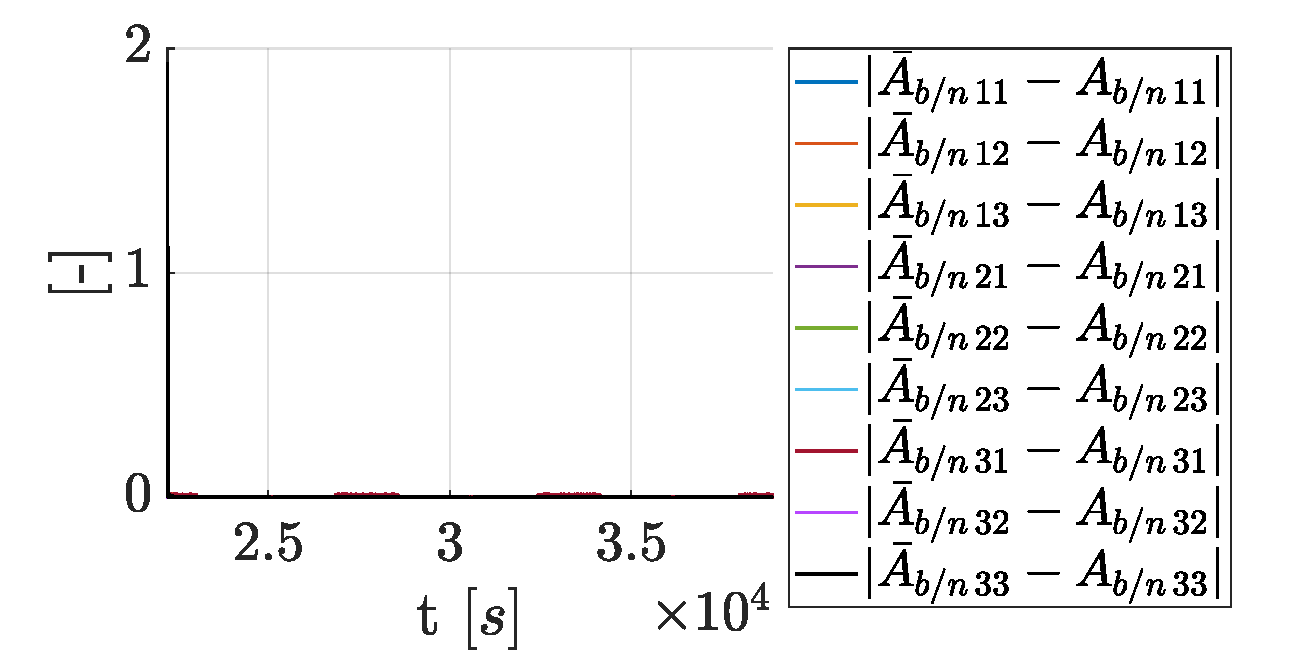
\includegraphics[width=0.49\textwidth]{graphics/tracking/tracking-estAbn.pdf}}
    \subfloat[Angular velocity]{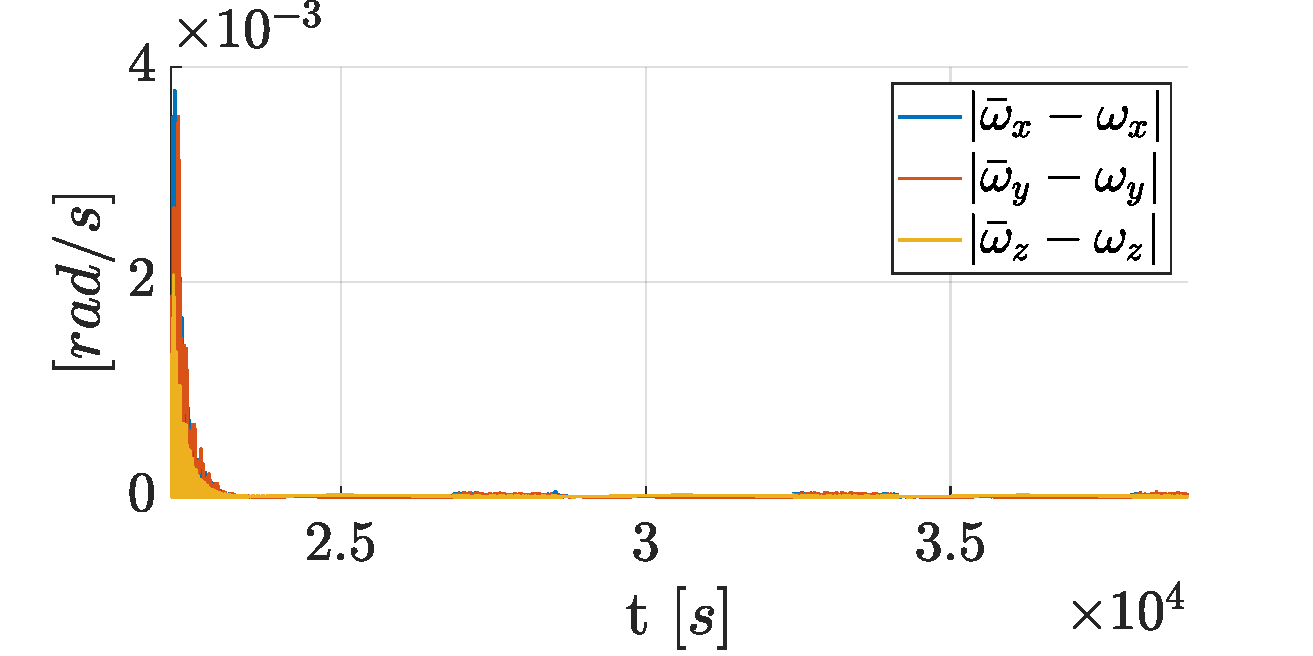
\includegraphics[width=0.49\textwidth]{graphics/tracking/tracking-estW.pdf}}
    \caption{Evolution of the estimation errors ($A_{b/n}$ and $\bm{\omega}$) in the tracking phase}
    \label{fig:tracking-estWabn}
\end{figure}   

\begin{figure}[h!]
    \subfloat[Disturbing torque \label{fig:tracking-estMd}]{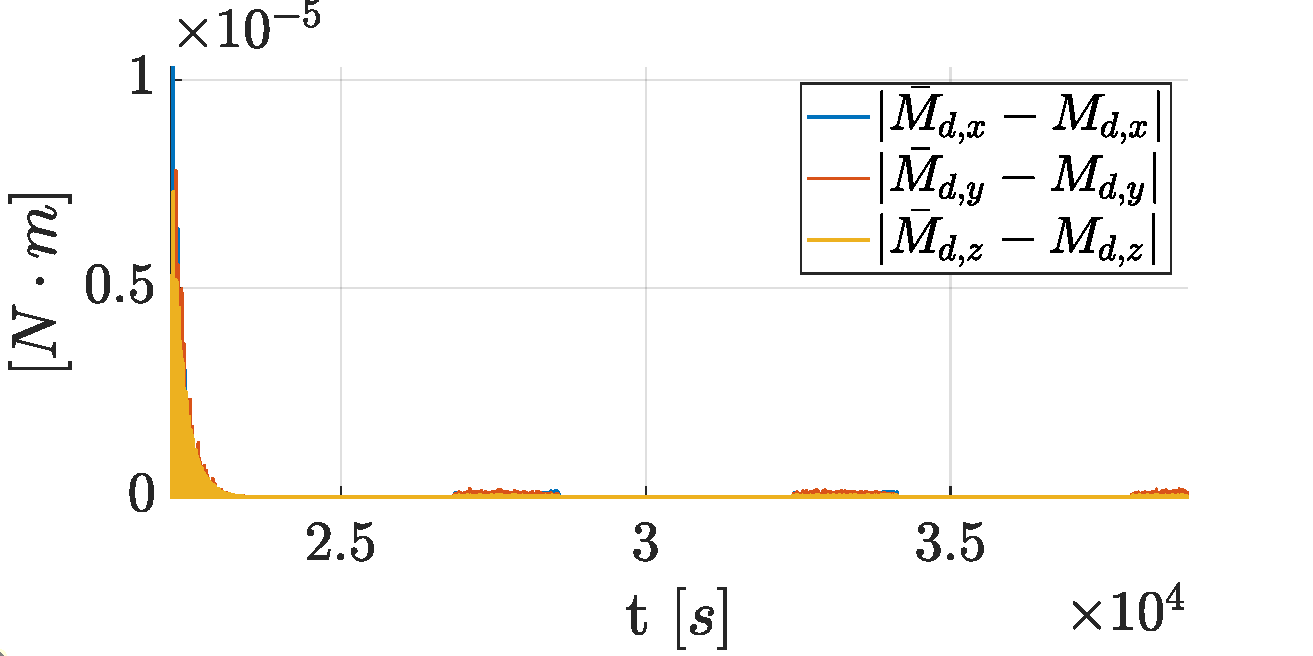
\includegraphics[width=0.49\textwidth]{graphics/tracking/tracking-estMd.pdf}}
    \subfloat[Control torque \label{fig:tracking-estMc}]{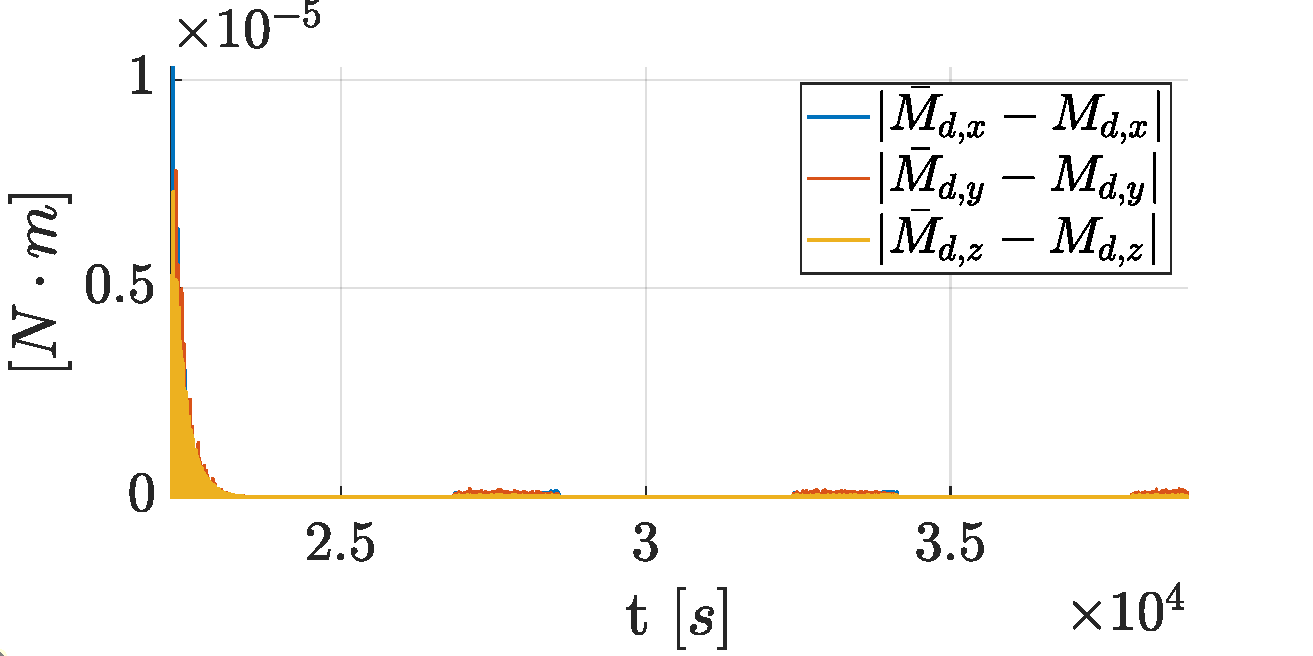
\includegraphics[width=0.49\textwidth]{graphics/tracking/tracking-estMd.pdf}}
    \caption{Evolution of the estimation errors ($\mathbf{M}_d$ and $\mathbf{M}_c$) in the tracking phase}
    \label{fig:tracking-estM}
\end{figure}

The maximum estimation errors on the torques (for $t > \bar{t} = 30482.89 \, s$) are presented in \cref{tab:torques_estimation}. The search region for the maxima is reduced in order to exclude the first time instants, in which the dynamics of the estimation is not settled yet. The error on the disturbing torque is approximately in the order of the torques itself (\cref{tab:magnitude_torques}). Nevertheless, it is possible to notice that this uncertainty is filtered out when estimating the control torque (whose error is extremely low), so it does not affect the robustness of the control system.

\begin{table}[h!]
    \centering
    \caption{Maximum estimation errors on the disturbing and control torques}
    \begin{tabular}{cc}
    \toprule
    \toprule
    $\max_{t > \bar{t}} \; \| \bar{\mathbf{M}}_d - \mathbf{M}_d \|$ & $\max_{t > \bar{t}} \; \| \bar{\mathbf{M}}_c - \mathbf{M}_c \|$ \\
    \midrule
    $2.02 \cdot 10^{-7} \, N \cdot m$ & $2.12 \cdot 10^{-20} \, N \cdot m$ \\
    \bottomrule
    \bottomrule
    \end{tabular}
    \label{tab:torques_estimation}
\end{table}

The angular momentum of the reaction wheels, whose evolution is reported in \cref{fig:tracking-hr}, oscillates periodically with monotonous increments of the DC offsets. The actuator will eventually reach saturation, hence a de-saturation mechanism shall be developed. On the other hand, the torque provided to the wheels $\mathbf{M}_r$ (\cref{fig:tracking-mr}) show a fast decay as the spacecraft reaches the desired attitude, after a first peak phase.

\begin{figure}[h!]
    \centering
    \subfloat[Angular momentum \label{fig:tracking-hr}]{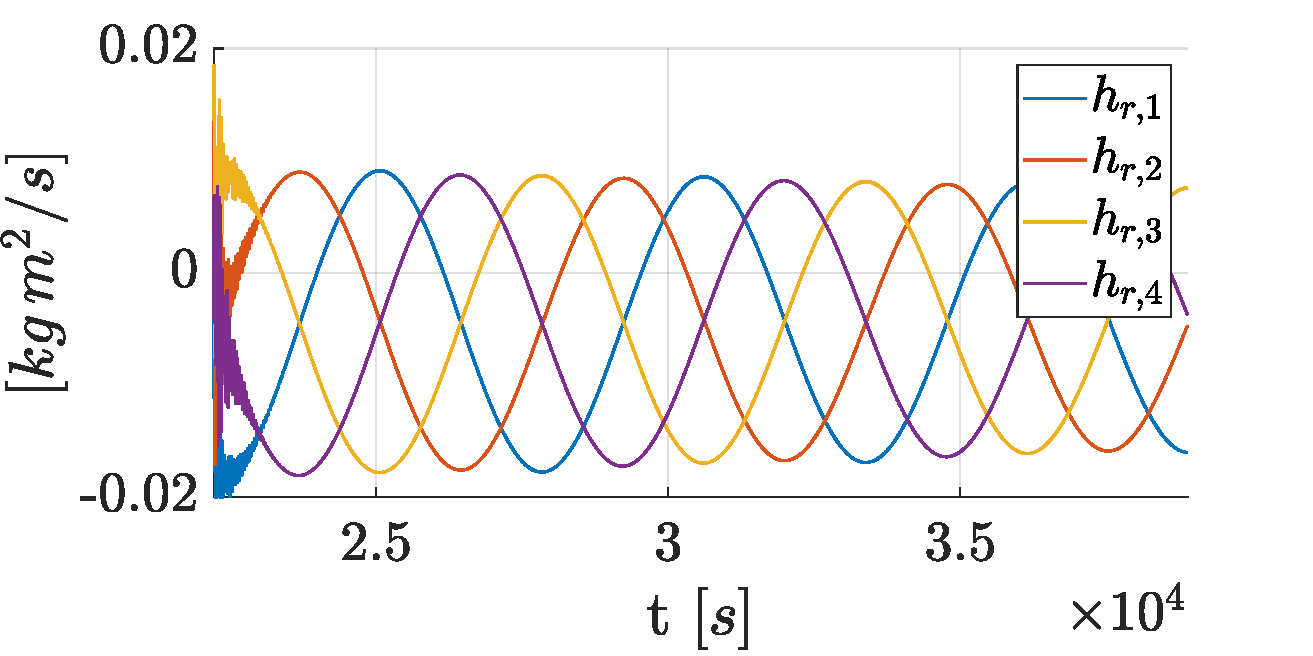
\includegraphics[width=0.49\textwidth]{graphics/tracking/tracking-hr.pdf}}
    \subfloat[Torque provided to the wheels \label{fig:tracking-mr}]{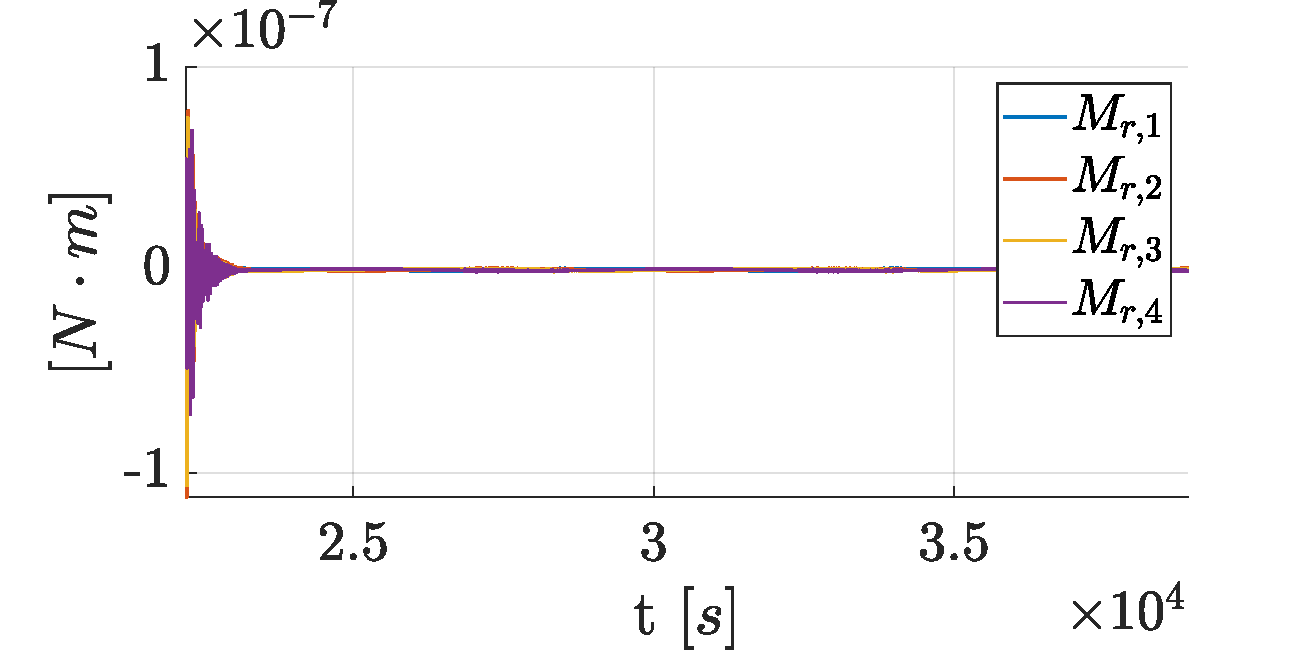
\includegraphics[width=0.49\textwidth]{graphics/tracking/tracking-Mr.pdf}}
    \caption{Evolution of $\mathbf{h}_r$ and $\mathbf{M}_r$ in the tracking phase}
    \label{fig:tracking-rw}
\end{figure}